\chapter{Discussion}

\section{Selecting Working Agreements}

As with any goal, Working Agreements should be achievable. Unrealistic targets tend to be ignored by the team members and can decrease motivation~\cite{forsgren_space_2021}. That said, it is valuable that teams configure Working Agreements on their own. Not all WAs are suitable for all teams: for example, branching strategy needs to be considered during the WA setup.  

Because Working Agreement templates are defined by Swarmia, the client teams have limited capacity to adjust or fine-tune WAs for their needs. Certain presumptions made might make the WAs less valuable or even unusable for some teams: to get the most value out of Swarmia, teams should work with widely accepted CI/CD practices. 

At the beginning of a customership, Swarmia helps clients to get the most out of the product. Swarmia employees showcase product features in these meetings and configure initial settings with client representatives. The intention is to get the team started swiftly and help them discover the most relevant features of the product.

An unsuccessful initial setup of Swarmia may cause unwanted effects. For example, a client CTO could be eager to do the initial setup for all teams at once without input from their leads or team members. As stated in Accelerate~\cite{forsgren_accelerate_2018}, this is a bad habit: teams should choose their tools and setup. In the onboarding sessions, Swarmia can guide the client representatives with the best practices for WA setup by involving the team leads in the onboarding process. Successful onboarding can form a sound basis for the setup sessions the teams should have on their own. 

It remains unclear how teams change their configurations over time. The working methods or changes made to them was not studied. For example, some teams create WIP-labeled pull requests to inform their teammates of their status or to discuss the upcoming changes. Such a habit leads to a large amount of open PRs and the team should adjust their WIP Working Agreement accordingly. To keep the Working Agreements achievable, teams should review and adjust them regularly. In this study, the models always used the most recent configuration, not the initial ones. This way, the effect of the potential adjustments was included. Intuitively, with periodical iterations to the agreements, teams should find the optimal setup. Unfortunately, the number of adjustments or their frequency remains unknown in this study. 

Working Agreements are not intended to be used as primary performance metrics but as a tool that helps teams achieve their objectives. Therefore, it is a safe assumption that teams aim to improve their productivity by enabling WAs. The two most popular WAs, max\_pull\_request\_review\_time and max\_pull\_request\_age, aim to reduce the pull request cycle time. It seems teams using Swarmia are keen on increasing their PR throughput. Additionally, many practices that WAs introduce are already used in the teams. By using Working Agreements, teams get up-to-date information on their track record and ensure that the rules are followed in the future. 

Most teams enable only a couple of Working Agreements: $64\%$ of teams have configured four or fewer agreements. Teams might test the feature with a couple of agreements and then decide to go all-in if the feature proves helpful. Furthermore, teams usually configure only one Working Agreement per template. A potential reason is related to feature discovery: the possibility of creating multiple agreements might need to be clarified for new teams. The fact that Story is the most popular issue type suggests that most Swarmia teams are acclimated to using Swarmia for Story tracking while Epics, Bugs, and Tasks are tracked via other tools like GitHub – or not at all.

\section{Effect of Working Agreements}

Next, we will analyze the independent variables with statistical significance in the PRCT and IPCT models and the potential underlying reasons for the perceived results. Then, the more specific targets the teams set for the agreements are analyzed.

\subsection{Effect of Working Agreement Setup}

Limiting the number of open PRs with wip\_pull\_requests does increase PRCT with a weight of 1.28 and notably high confidence. This means that the PR age would increase by 1.3 days. Especially interesting is that it also increases IPCT, the actual development time, by one and a half days. By introducing this working agreement, teams try to limit pull requests on their desk. As the agreement does not directly control the amount of open PRs, it should not form a bottleneck. In other words, as the agreement is not forced, the effect on developer behavior is indirect: nothing prevents them from creating more PRs than the set maximum in the WA configuration. 

To get a deeper insight into the pull request WIP limit, we reflect on the results using Little's law~\cite{chhajed_building_2008}. The law can be formulated $L=\lambda W$, where $L$ is the number of items in the system, $\lambda$ is the arrival rate, and $W$ is the average time items spend in the system. In this context, we can denote $W=T_{IRCT}$, the average time it takes to review a pull request. As now $W=L/\lambda$, an increase in $W$ would mean that either $L$ has increased or $\lambda$ has decreased. Based on Little's law, setting a WIP working agreement for pull requests should decrease $L$ and therefore decrease IRCT, given that the arrival rate does not also decrease in the process. 

The results for wip\_pull\_requests conflict with Little's law: no relationship between IRCT and working agreement setup was found. On the other hand, trying to limit the number of PRs in the system $(L)$ caused an increase in PRCT and IPCT. As no relationship between IRCT or RMCT and WA setup was found in the models, it can be assumed that the increase in PRCT resulted from increased IPCT: the developers work on pull requests longer. It seems that the PR limit can result in a larger batch size; the number of changes in a PR increases, which prolongs the development time, IPCT. 

While literature suggests that WIP limits are suitable for team productivity~\cite{reinertsen_principles_2009}, in some teams, their overall processes do not support using them. A potential solution would be to intervene earlier before the limit is exceeded. The solution could be implemented with more proactive notifications or inbuilt limits that disable creating new PRs before the old ones are reviewed and merged. Similar limits are already used in, e.g., GitHub: for example, a team can set a requirement for peer approval before a PR is merged.

By discouraging pushing to the main branch, team members are expected to work through pull requests instead of blindly merging their changes to the main branch. The results imply a strong decreasing effect on both PRCT and IPCT, with the respective weights $w=-1.28$ and $w=-1.01$. Practically speaking, this would shorten PR age by 1.3 days and development time by a day. These results could be caused by creating a superficial working habit: the teams implement a system where pull requests are created but approved without a proper review. In other words, PRs are made for each change to comply with the working agreement and potential branch protection rules. These for-the-sake-of-it PRs pull down the PRCT: without the WA, PRs probably were made only for the more extensive changes. Even though the rule creates more friction between development and merging to main, reviewing all changes is considered a good practice and should increase code quality. Furthermore, even the rubber-stamped PRs are net-positive for the change history. To get a better touch of this working agreement's potential, we would have to use more relevant metrics, such as the change failure rate. 

Pull request review times are considered a common bottleneck in software development~\cite{maddila_nudge_2022}. By enabling max\_pull\_request\_review\_time, teams try to encourage themselves to focus on closing open PRs faster. Often review times can prolong due to the inactivity of the author or the reviewer. The result, a decrease of 0.81 days in PRCT, proves that the WA reduced review times by almost a day. An interesting result is that the WA also decreased IPCT by $-1.51$ days: this indirect effect could be caused by the teams' need to decrease the batch size, which should lead to quicker PR reviews. These smaller batches spend by average 1.5 days less time in progress.

Furthermore, max\_pull\_request\_review\_time is the only WA the personal Slack notifications address: each team member can opt-in to receive direct messages for PRs pending their contribution. The team daily digest also lists open PRs on top, again bringing them to the attention of developers. According to~\citet{maddila_nudge_2022}, actively notifying developers of open PRs shortens PR review time.

\begin{figure}[ht]
    \centering
    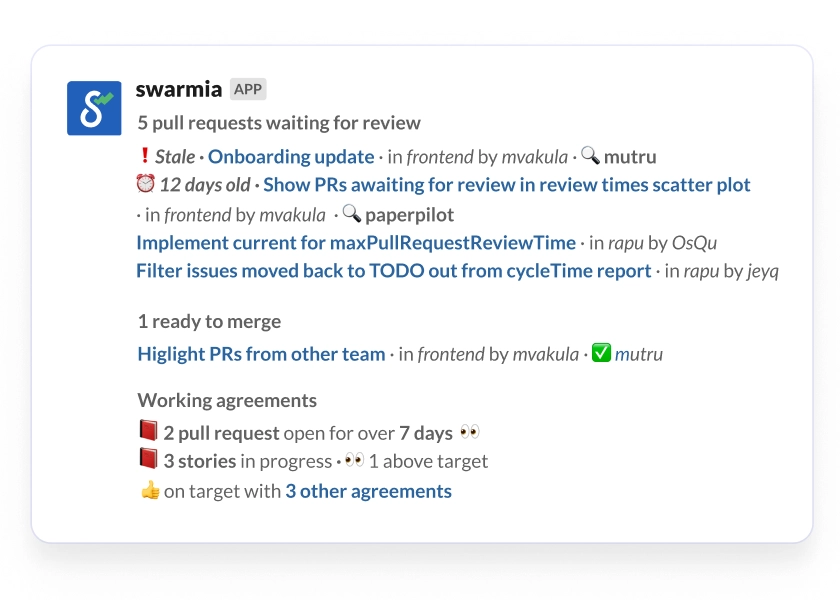
\includegraphics[width=13.5cm]{LaTeX/images/daily-digest.png}
    \caption{Daily Digest, a status report posted by the Slack integration}
    \label{fig:daily_digest}
\end{figure}

The rest of the WAs proved no results in these models that could be trusted due to the lack of statistical significance. Not all Working Agreements aim to reduce cycle times directly, and consequently, there will not be a direct connection. An interesting phenomenon is that PRCT does not have a relationship with any of the issue-related WAs: even though it is a PR-related metric, one would intuitively expect there to be a connection with, for example, wip\_issues and PRCT. 

\subsection{Effect of Working Agreement Targets}

Finally, the effect of Working Agreement targets is analyzed. The target models for PRCT and IRCT yielded significant results. In these models, the independent variable was modeled as a Boolean metric, as we did not want to give additional weight to the subtraction of target and result: it only matters whether the team achieved their goals. For example, if the team sets their target of PRCT to seven days, both cycle times of five or six days can be seen as evenly valuable results.

The target for the WA, denoted with target\_days, has a strong positive effect on the goal achievement. In other words, by setting more loose goals, the teams reach these goals more often. The result is intuitive: with more time to spend, it is easier to be on time. On the other hand, the weight of the effect provides deeper insight: for PRCT $w=0.0144$ and for IRCT $w=0.0978$. Therefore, a ten-day limit for PRCT would affect $0.144$ on whether the goal is met. Again, considering that the independent variable has Boolean values,  it can be stated that the effect is minor. Furthermore, a typical PRCT limit is measured in weeks and an IRCT limit in days, so even a ten days increase would be considered significant.

This result is in line with Parkinson's law: a task tends to take the time allocated for it~\cite{parkinson_cyril_parkinsons_1955}. Although, a smaller target can motivate teams to work in smaller batches so that the task at hand might change: for example, a Jira issue might be split into three PRs instead of one, while the overall complexity and time spent might be the same. Unfortunately, the PR contents were not analyzed, so the agreement's effect on batch size remains unknown.

On the contrary, a decreasing effect on the independent variable can be seen with days\_in\_use, the number of days since WA activation. The weights are for PRCT $w=-0.000234$ and for IRCT $w=-0.000128$. Even though the effect is arguably tiny, it does accumulate over time: the teams are expected to use the product for years, so the weights can become even thousandfold.

\section{Studying Teams and Individuals}

SPACE divides productivity metrics into three levels: individual, team, and system~\cite{forsgren_space_2021}. Of these, this study focuses on the team level while also including some aspects from the individual viewpoint. Next, we will review the findings related to three metrics that deal with teams and individuals: slack\_users, github\_authors, and daily\_digest.

The number of weekly PR authors, which we assume correlates strongly with team size, did not have a relationship to the cycle times and was, in the end, removed from the models due to an excessively high correlation with slack\_users. 

In previous work, authors have argued that smaller software development teams boost individual performance and operate with smaller total effort~\cite{sutherland_teams_2014, mundra_practical_2013}. Although larger team size and changes in team composition are often considered performance degrading factors, the results indicate that team size and cycle times have no direct connection.

Regarding the team-level results, we must highlight that we use metrics that not all teams aim to improve while others actively do. As metrics influence behavior~\cite{forsgren_space_2021, storey_how_2022}, the teams that measure cycle times daily might perform differently from those that do not. 

\subsection{Team Metrics and Pull Request Cycle Time}

As for the PRCT model, slack\_users has a weight of $-2.45$ hours per user. For a five-person team, this means that if each team member enables Slack notifications, PRCT decreases by 12 hours. The Slack messages nudge the individuals to review their peers' pull requests, reducing the gap between review request and change approval, a common gatekeeper for merging the change. 

On the other hand, the team-wide notification Daily Digest does not influence PRCT. Teams integrate the Daily Digest into their current communication channel or create a dedicated channel. As with any high-volume medium, these channels can be flooded with content, causing the notifications to be missed or ignored by the team members.

The direct message continues to be an efficient way to reach individual contributors. Companies implementing direct message notifications should be careful to refrain from spamming developers needlessly~\cite{maddila_nudge_2022}. Based on these results, Swarmia has created a valuable personal notification experience. 

\subsection{Team Metrics and In Progress Cycle Time}

For the IPCT model, the situation is the opposite: slack\_users does not have statistical significance, but daily\_digest does, with $w=-0.595$. The result implies that team-level notifications decrease a single PR's development time by 0.6 days, while personal notifications have no effect. The lack of relationship between slack\_users and IPCT is as expected: the direct message notifications only deal with the steps after opening a PR when IPCT has ended. The Daily Digest instead includes information about ongoing development tasks: the issues in progress are fetched from the issue tracker and summarized in this report. 

The reasons behind this effect could be associated with peer pressure. Posting a public report daily to the Slack channel, the Daily Digest surfaces each issue's status for the team. Although teams can go through the same topics manually in the daily standup, the Daily Digest makes this update more structured and based on actual issue tracker data. The practice should create a positive sense of urgency for the individual contributors, and increase the development speed. Additionally, the team members can notice bottlenecks earlier and support their peers. 

As slack\_users correlates strongly with team size, it is interesting to notice how it has a decreasing effect on PRCT but not on IPCT. To generalize, the number of team members shortens the average pull request lifetime without affecting the actual development time. The gains are therefore found in the post-development steps: code review and merge. It seems that larger teams can find time to review each other's code with less lag and merge the changes faster after a green light from the reviewer. 

Prior empirical research has shown that increasing team size does not linearly increase development cost~\cite{pendharkar_relationship_2009} and that teams with less than nine members tend to be more productive overall~\cite{rodriguez_empirical_2012}. Furthermore, Heričko et al. argue that for each project, there exists an optimal team size~\cite{hericko_approach_2008}. The results found here can provide direction for future research to determine in which stages the larger team size can be beneficial.

\subsection{Targets and Team Metrics}

The team metrics were used as dependent variables in the target models. Again, these weights should be interpreted with the Boolean dependent variable in mind, not as days as in the previous results. The usage of Daily Digest did not have a statistical correlation for either of the targets researched. This result is in line with the previous findings: Daily Digest does not influence PRCT or IRCT directly but affects IPCT. These results further highlight the lack of statistical connection between Daily Digest and the targets the teams have set for PRCT and IRCT with the associated WAs, even though the Daily Digest especially emphasizes showcasing how teams are doing with their targets. 

On the other hand, the effect of slack\_users can be seen in these models, which is surprisingly contradictory with the previous results: the number of Slack notification users decreases whether the goals were met. The results are for PRCT $w=-0.00551$ and IRCT $w=-0.00463$, with a slightly negative impact on both. Especially the results regarding PRCT targets raise questions, as we have seen a positive effect with the PRCT itself and slack\_users but not with the PRCT-related target.

Based on the results, larger teams perform better in terms of pull request cycle time but miss their targets related to it more often: they set too ambitious targets while performing quite well in absolute metrics. The added complexity of more team members might cause this, as it makes estimation harder. 

\section{Directions for Future Work}

In Accelerate, the authors argue~\cite{forsgren_accelerate_2018} that teams should be able to choose their methods and tools. Even though the study only handles monthly active users, it is hard to know their commitment to Swarmia: did they collectively decide to use such a tool and if they did, were the Working Agreements selected as a team or by a manager. The results could improve organization and team onboarding for various SaaS tools. 

Moreover, the teams' overall motivation for improvement remains to be discovered. The perceived need for change within the team plays a crucial role in the success of organizational change~\cite{lenberg_initial_2017}. The teams' background, focusing on the individual contributors' views on change, could provide more depth to the analysis. Additionally, the effect of the organization characteristics remains to be discovered: for example, companies with different technology stacks, amount of technical dept, or type of product might benefit from a different WA setup.

One of the key findings, the effect of slack\_users, would deserve further analysis. Currently, personal notifications are measured on the top level: whether they are used or not. Variations of the notification could be researched to understand better which notifications have an impact. Future studies could include comparing competing tools, such as GitHub's Slack integration~\cite{slack_technologies_integrationsslack_2022}, Microsoft's Nudge Service~\cite{maddila_nudge_2022}, and Swarmia. Furthermore, the length of the effect would need further validation – is the boost achieved by using Slack notifications persistent.

The most exciting direction of further research is tracking the ways of working that, at the time of writing, can not be configured with Swarmia. These norms can be implemented very differently in teams and are more challenging to track objectively than the WAs in Swarmia. However, they admittedly make up most of the teams' ways of working. For example, potential themes for these so-called non-technical Working Agreements could be meeting practices or communication guidelines.

\section{Limitations of Work}

Regarding internal validity, there are a few relevant remarks. Most notably, this thesis uses cycle times as the primary metric. Even though reducing cycle times is a goal many teams try to achieve, there are also potential downsides, such as reduced code quality. Frameworks like SPACE and DORA metrics highlight the need for multiple team productivity metrics to find an optimal balance: a single activity metric cannot reflect all relevant aspects. For example, the change failure rate, which Swarmia already calculates for the customer teams, would bring more depth into the analysis. Furthermore, self-reported measures such as whether an engineer felt productive today, would be a needed counterweight for activity metrics.  

Linear regression models were used, even though $cycletime > 0$ always: the dependent variable would be truly continuous in an ideal situation. Furthermore, the factors used as independent variables cannot be considered to constitute all the potential factors that may influence PRCT. Factors such as team members' experience or whether teams operate remotely could affect team productivity but were not included in this study. When using a linear model, it is worth noticing that the relationship between independent and dependent variables will not be linear indefinitely. For example, even though adding another Slack user reduces PRCT by 2.45 hours, it does not mean that adding 1000 new users reduces the time by thousands of hours. 

As this is a quantitative study, we rely solely on data available on Swarmia business intelligence tools. Conducting user interviews or surveys would unlock many avenues currently only asserted speculatively. For example, studying perceived performance is more labor-intensive but can shed light on otherwise hard-to-measure dimensions. How people feel they are making progress is a proxy of productivity~\cite{forsgren_space_2021}. A positive attribute of the study is that it was conducted using historical data: the teams were unaware that their usage logs would be used as thesis material.

Regarding external validity, there are multiple weak points in the study setting. Although we set out to investigate how the Swarmia sub-feature affects team behavior, the aim is to be able to generalize the findings to any other ways of working system. Using Swarmia's Working Agreements is presumably more effective than non-technical implementations, as it actively keeps track of the agreements and nudges team members to stay on track. Regarding generalizability, the results achieved in this study are not directly derivative of other team norm systems. Furthermore, a tool like Swarmia attracts certain companies more than others, causing selection bias for the study. If these organizations are willing to invest in such a tool, they might have more motivation to improve than the companies that decide against using Swarmia or similar tools. 

The two-year data collection period overlaps significantly with the coronavirus pandemic, which more or less affected any technology company. Changes like layoffs, remote work, or pivots cause significant effects on team dynamics. These probable effects must be considered with the available data. Even though Swarmia's client base is international and consists of all kinds of companies, the effect of a pandemic can not be ruled out completely.